\section{Integration between virtual and physical networks}

The integration between underlay and overlay networks aim to allow multiple virtual networks, or tenants, to communicate over the physical IP fabric on a spine–leaf topology in an isolated and efficient manner. The underlay, representing the physical fabric, provides predictable transport mechanisms, such as ECMP and rapid convergence, while the overlay provides isolation and operational agility. The convergence of these two domains occurs at the network virtualization edge (NVE), typically located at the rack level, where a virtualization endpoint, such as a VXLAN VTEP or Geneve GTEP, performs encapsulation and decapsulation. From the VM's perspective, this process is transparent, as frames are sent and received as if within a traditional LAN.

Coherency between the logical and physical planes is maintained through an explicit control plane. In modern data center environments, Ethernet VPN (EVPN) based on BGP disseminates reachability information, informing each NVE of the MAC and IP addresses, the corresponding virtual network identifiers and their location within the fabric. This mechanism enables direct encapsulation to destination nodes, eliminating the need for broadcast, unknown-unicast, and multicast traffic through formal advertisements and ARP/ND suppression. Furthermore, EVPN supports the integration of Layer 2 bridging and Layer 3 routing through integrated routing and bridging and anycast gateway functions, ensuring that the first routing hop occurs locally.

The meeting point between physical and virtual domains materialized at the NVEs, whose placement conditions the division of functions without altering the logical model. As illustrated in Figure~\ref{NVEplacement}, NVEs can be implemented either on the hypervisor or on the leaf switch, each approach presenting distinct trade-offs in terms of performance, flexibility and integration with the physical fabric. 

\begin{wrapfigure}{r}{0.45\textwidth}
    \vspace{-15pt}
    \centering
    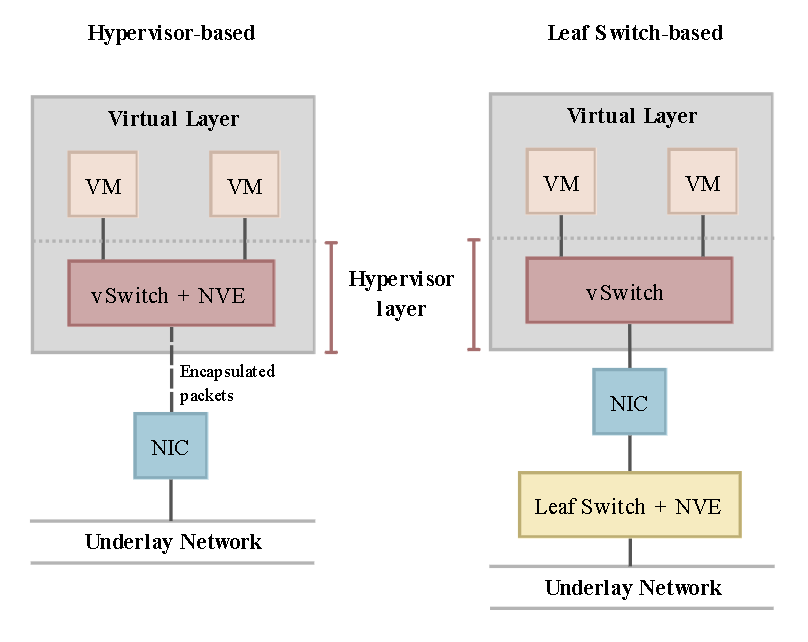
\includegraphics[width=\linewidth]{Figures/NVEplacement.png}
    \caption{NVE placement.}
    \label{NVEplacement}
    \vspace{-5pt}
\end{wrapfigure}

When the NVE is implemented on the hypervisor, the virtual switch, like OVS or NSX vSwitch encapsulates VXLAN or Geneve and, if applicable, acts as a distributed gateway. The resulting IP/UDP packet leaves the server network interface and the leaf carries it over the underlay to the destination NVE. Physical switches are not required to understand the overlay, although many modern platforms natively support it. This approach offers flexibility and independence from hardware capabilities but consumes host CPU resources for encapsulation, decapsulation, and local routing.

Contrarily, when the virtualization edge resides on the leaf switch, the VM transmits a regular Ethernet frame to the virtual switch, the leaf identifies the associated VNI and performs hardware-based encapsulation at line rate, also acting as an anycast gateway per virtual network. The encapsulated VXLAN or Geneve packet is then forwarded across the fabric to the destination leaf. This design offers lower latency, minimal jitter, and improved integration with bare-metal workloads through direct VLAN-to-VNI mapping at the network edge.

In summary, integrating physical and virtual networks consists of separating responsibilities (transport vs. segmentation/policies) and synchronizing state with a robust control plane, such as EVPN. Thus, the physical fabric remains simple and scalable, while the virtual plane gains the flexibility needed to host many tenants and move workloads without friction.

